\subsection{Planet Yield from the Primary Mission}
\label{sec:results_from_primary_missions}
\begin{marginfigure} %[t]
	\centering
	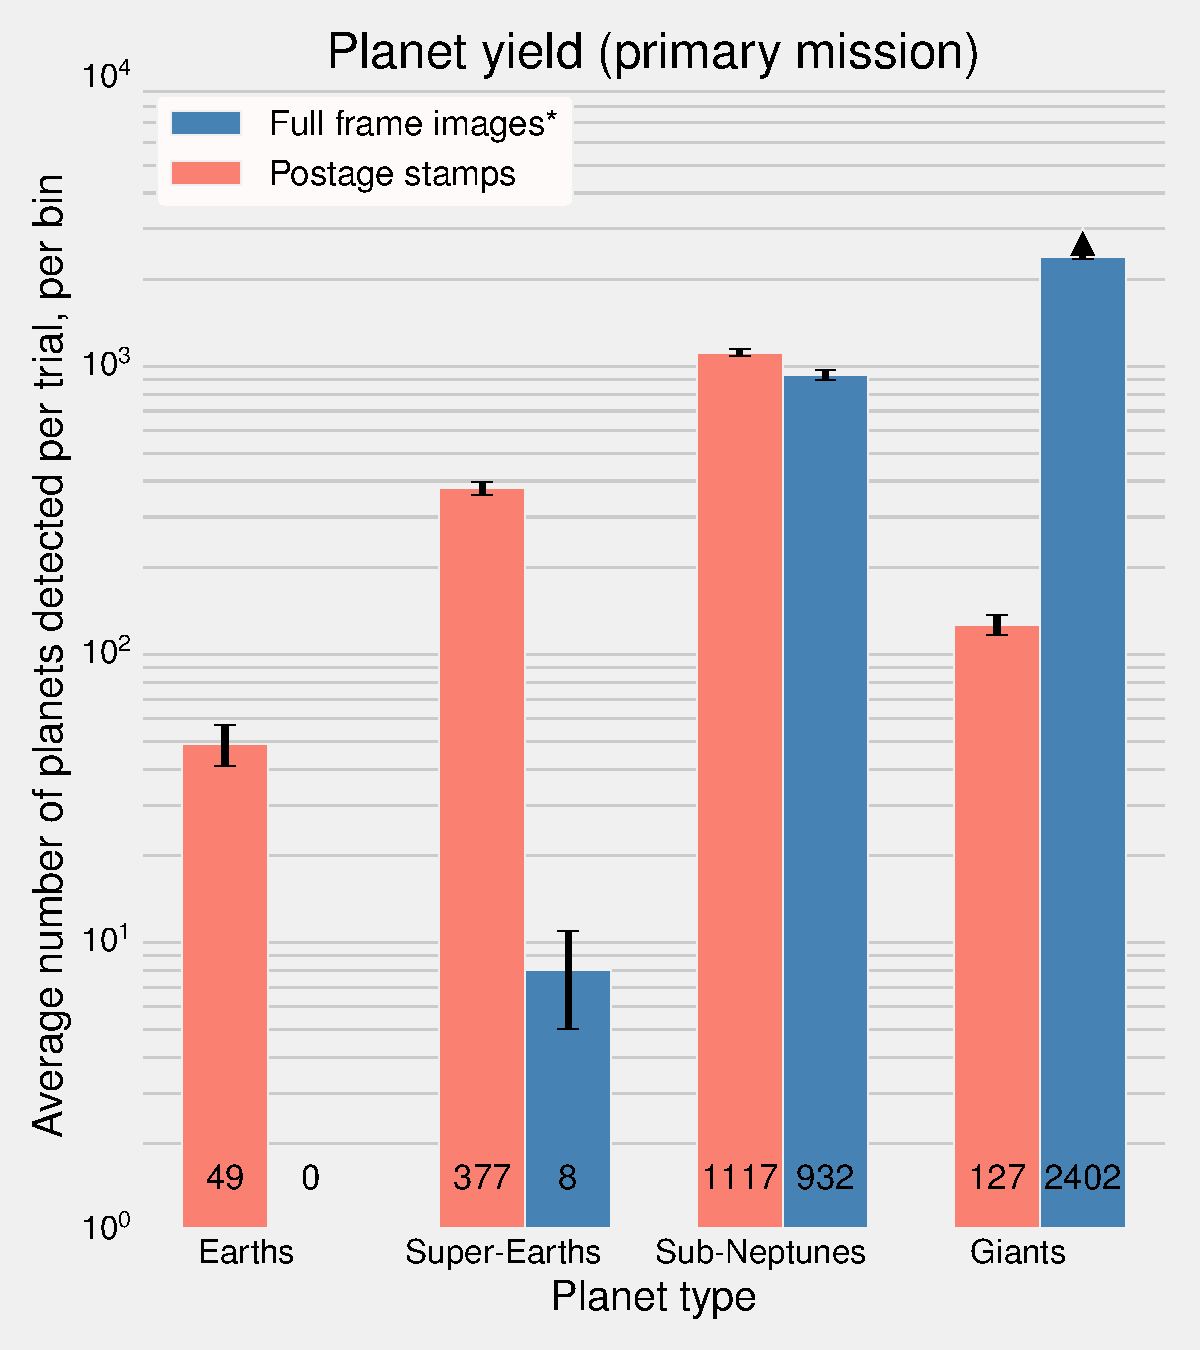
\includegraphics[width=\textwidth]{figures/160729_pm0_shemi_nhemi_nhemi_t50-pri_bar_chart.pdf}
	\caption{Mean numbers of planets detected in \tesss Primary Mission.
	The number of Earths ($R_p < 1.25R_\oplus$), super-Earths ($1.25R_\oplus \le R_p < 2R_\oplus$), sub-Neptunes ($2R_\oplus \le R_p < 4R_\oplus$) and giants agree with the respective values quoted in \protect\citet{Sullivan_2015} to $\lesssim 50\%$. 
	%despite modifications to our target selection procedure (Sec.~\protect\ref{sec:selection_criteria}).
	Our full frame images detections are complete for $R_p < 4R_\oplus$, and 
	incomplete for giant ($R_p > 4R_\oplus$) planets, shown with a lower limit 
	(see text for discussion). 
	Error bars are from only Poisson fluctuations and do not account for systematic uncertainty.}
	\label{fig:primary_planet_yield}
\end{marginfigure}
We first examine our results for just the Primary Mission -- the first two years of \tesss observing. 
We follow with an analysis of our detected planet populations from a single Year-3 Extended Mission (Sec.~\ref{sec:results_from_nhemi_extended_mission}), and then all six of our proposed Extended Missions (Sec.~\ref{sec:results_from_all_extended_missions}).
Here we highlight commonalities and differences between~\citetalias{Sullivan_2015} and this work.

\paragraph{Detected planet yield}
The first point of consideration is the detected planet yield, shown in Fig.~\ref{fig:primary_planet_yield}.
The number of Earths, super-Earths, and sub-Neptunes we detect agrees with the 
numbers quoted by~\citetalias{Sullivan_2015} to within $50\%$, despite the 
modifications described in Sec.~\ref{sec:selection_criteria} to the target 
selection procedure.
Other changes to our simulation's assumptions, for instance using an as-built 
model of \tesss PSF informed by laboratory tests (courtesy Deborah Woods) 
rather than the idealized PSF described in Sec 6.1 
of~\citetalias{Sullivan_2015}, had only minor impact on this final result 
($10\%$ change in yield).

In the preparation of this report, a
discrepancy emerged between our predicted $\approx 400$ super-Earth detections 
and those shown in Fig.~18 of~\citetalias{Sullivan_2015}, which 
displayed $\approx1400$ planets. The subsequent investigation led to the 
discovery of a bug in the plotting script used to create 
\citetalias{Sullivan_2015}'s Fig.~18 (an Erratum has been published). The 
error did not
affect any of the results described in~\citetalias{Sullivan_2015}'s text, or 
the simulation results that were tabulated in the paper and sent electronically 
to interested parties.
The corrected version 
of~\citetalias{Sullivan_2015}'s Fig.~18 shows $\approx 500$ expected 
super-Earths, which closely agrees with our work when also accounting for the 
dilution error described below.

Another modification was the correction of a bug in the dilution calculations
of~\citetalias{Sullivan_2015}. A single missing symbol\footnote{An $\texttt{=}$ rather than 
a $\texttt{+=}$} led~\citetalias{Sullivan_2015} to under-account for this 
effect. After correcting this error, the simulations yielded
about 30\% fewer Earth-sized and super-Earth planets than reported by \citetalias{Sullivan_2015}.

\paragraph{Properties of planets detected in Primary Mission} 

We show the population properties of planets detected in postage
stamps and full frame images during the Primary Mission in
Figs.~\ref{fig:radius_vs_period_nhemi}
and~\ref{fig:imag_vs_teff_nhemi}.  In terms of the apparent planet
radii $R_p$, orbital periods $P$, host star brightness, and host star
$T_\mathrm{eff}$, we qualitatively agree with the results
of~\citetalias{Sullivan_2015} for the planets detected
in postage stamps. 
For instance, the dearth of $P<5$ day
Neptune-radius ($R_p \lesssim 4R_\oplus$) planets in 
Fig.~\ref{fig:radius_vs_period_nhemi} was
observed by \textit{Kepler}~\citep{mazeh_dearth_2016}, and thus it is
present in our input occurrence rates, rather than being an
observational bias.  It was also seen by~\citetalias{Sullivan_2015}.

The differences between planets detected in postage stamps vs. in full frame images follow our expectation from our \texttt{Merit} statistic. 
Namely, Fig.~\ref{fig:imag_vs_teff_nhemi} shows that at a fixed brightness, full frame image detections tend to occur at larger stellar effective temperature (and thus stellar radius).
At a fixed host star radius, postage stamp detections occur around brighter stars.

\paragraph{Impact of earth and moon crossings on Primary Mission's detected planet yield}
During the Primary Mission, of the four cameras, Camera 1 (closest to the 
ecliptic) suffers the most from Earth and Moon crossings.
As noted in Table~\ref{tab:dropped_fields}, we remove 4 of its 13 
`observing sectors' from that year.
This reduces the number of planet detections near the ecliptic, and is visible in the orange points of Fig.~\ref{fig:skymap_nhemi}.
In the Primary Mission \tess detects $\sim20$ planets with $R_p<4R_\oplus$ 
(PS+FFI) in each $24^\circ\times24^\circ$ camera field nearest to the ecliptic.
As implemented in our simulation, Earth and Moon crossings result in some 
fields simply not being observed, so in these cases planets orbiting stars in 
these fields are never detected.
Considering only the Primary Mission, we would naively expect that dropping a total of 9 fields over the two years (again, see Table~\ref{tab:dropped_fields}) would result in a loss of $\sim9\times20=180$ planets.
This agrees with what our simulations actually give: running them without accounting for Earth and Moon losses returns a mean of 2678 detected planets with $R_p<4R_\oplus$, while running them with Earth and Moon crossings gives a mean of 2482 such planets (a loss of 196 planets; $7\%$ of the $R_p<4R_\oplus$ planet yield).
% data from 160708-t50 and 160729-t20. Slightly apples to oranges because of number of trials difference, but makes the point. 
